\chapter{Продукты}
\section{Неожиданная информация о вашей ежедневной еде}
\subsection{Сахар}
\begin{wrapfigure}{r}{0.5\textwidth}

\includegraphics[width=0.5\textwidth]{img/sugar.png}
    \caption{\textit{Исследования показывают, что слишком большое потребление сахара может привести к нездоровому питанию. Употребление сахара вызывает у многих людей желание есть еще больше сахара, что может привести к привычке переедания.}}
\end{wrapfigure}
Под сахором обычно понимают столовый сахар, химически известный как сахароза. Самые ранние известные свидетельства производства сахара поступают из Индии, примерно в 500 году до нашей эры. Исторически сахар использовался в нерафинированном сыром виде, полученном непосредственно из сахарного тростника. Стебли сахарного тростника взбивали, чтобы извлечь сок тростника, который затем осветляли и кипятили до кристаллического состояния.

Затем твердое вещество разбивали на мелкие кусочки и использовали в таком виде. На самом деле слово “сахар” происходит от санскритского слова sharkara, что буквально означает “галька". Сахарный тростник был относительно неизвестен на Древнем Западе. Одним из первых греков, столкнувшихся с сахарным тростником, был Неарх, командующий армией Александра. Во время своих путешествий по реке Инд он описал тростник, который производил мед без пчел!

Сегодня большая часть коммерчески доступных сахаров химически очищается и перерабатывается из его сырого формата. По данным Национального института здравоохранения Соединенных Штатов, такой рафинированный сахар --- это “пустые калории”, поскольку в процессе рафинирования удаляются почти все витамины и минералы, что резко снижает питательную ценность сахара \cite{Carbohydrates}.

Американская ассоциация сердца проводит различие между "внутренним" естественным сахаром, который относится к сахару, содержащемуся в природе как неотъемлемый компонент фруктов, овощей и молочных продуктов, и "внешним" добавленным сахаром, который относится к сахарозе или другим рафинированным сахарам, добавляемым в безалкогольные напитки, продукты питания и фруктовые напитки. Их исследование обнаружило, что есть вероятность того, что высокое потребление сахара может усугубить атеросклероз и способствовать развитию диабета и дефицита питательных веществ \cite{SugarCardiovascular}.

\section*{Лучше попробуйте это}
\subsection{Джаггери}
Хорошим заменителем сахара является джаггери. Джаггери~--- это нерафинированная, необработанная форма сахара, которая использовалась древними и привела Неарха в замешательство, когда он увидел ее. Джаггери широко используется в Индии и Южной Азии в качестве подсластителя. Он сохраняет минералы, питательные вещества и витамины, содержащиеся в соке тростника, и используется в Аюрведе~--- древней индийской медицинской системе~--- для лечения сухого кашля, улучшения пищеварения и против множества других проблем со здоровьем.

\begin{KeepInMind}
Некоторые продукты, продаваемые как джаггери, содержат химическое вещество под названием суперфосфат, которое наносит вред здоровью. Белый, аккуратный джаггери~--- это суперфосфатный джаггери, которого следует избегать. “Уродливый”, темный на вид джаггери обычно является правильным джаггери.
\end{KeepInMind}

\subsection{Мед}

\begin{wrapfigure}{r}{0.5\textwidth}
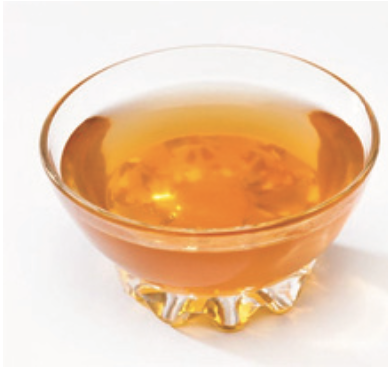
\includegraphics[width=0.5\textwidth]{img/honey.png}
    \caption{\textit{Чтобы собрать 1 кг меда пчелы путешествуют 195'000 км, что состовляет примерно 5 оборотов вокруг земли.}}
\end{wrapfigure}
Мед также является прекрасным заменителем сахара. Ежедневное потребление меда может сильно повысить здоровье, особенно у людей с проблемами избытка слизи и астмой. Это также очень полезно для сердца и мозга, а также сохраняет бдительность ума.

Мед был отмечен за его положительное влияние на здоровье в нескольких древних медицинских текстах. Современные исследования также сосредоточены на лечебных свойствах меда и дают несколько интересных результатов. Когда мед смешивают с теплой водой и употребляют каждый день, он повышает количество эритроцитов (RBC) в системе кровообращения. Эритроциты являются основным средством доставки кислорода к различным частям тела. Потребление меда также способствует увеличению полезных антиоксидантных веществ, активизирует антитела и борется с вредной микробной активностью \cite{EffectHoney} \cite{HoneyMicrobial}.



